\section{Resultados}\label{sec:resultados}

\subsection{Comparación de modelos}

La Tabla~\ref{tab:modelos} reúne el RMSE de nivel de cada modelo en los escenarios de validación, y la
Fig.~\ref{fig:exclusion} muestra cómo crece con la zona de exclusión.

\begin{table*}[t]
\centering
\caption{RMSE de nivel municipal (t/ha), media de 10 repeticiones. Pond. indica ponderado por superficie sembrada.
En negritas, el menor de cada columna. n.d. indica que el modelo no se evaluó en ese escenario.}
\label{tab:modelos}
\footnotesize
\begin{tabular}{@{}lcccccc@{}}
\toprule
 & \multicolumn{2}{c}{$B = 0$\,km} & \multicolumn{2}{c}{$B = 50$\,km} & Por distrito & Sin repetidos, $B = 0$ \\
\cmidrule(lr){2-3}\cmidrule(lr){4-5}
Modelo & Pond. & Sin ponderar & Pond. & Sin ponderar & Pond. & Pond. \\
\midrule
Media global & 0.504 & 0.488 & 0.594 & 0.579 & 0.534 & 0.592 \\
Media estatal & 0.451 & 0.410 & 0.644 & 0.530 & 0.497 & 0.532 \\
IDW de vecinos & 0.349 & 0.349 & 0.560 & 0.510 & 0.446 & 0.402 \\
Kriging de vecinos & 0.309 & \textbf{0.343} & 0.566 & 0.518 & 0.503 & 0.402 \\\midrule
Tmax jul-ago & 0.334 & 0.457 & 0.490 & 0.511 & 0.373 & 0.422 \\
Elevación & 0.437 & 0.509 & 0.631 & 0.623 & 0.481 & 0.546 \\
Tmax y lluvia & 0.272 & 0.426 & 0.506 & 0.515 & \textbf{0.305} & \textbf{0.365} \\
Tmax, lluvia y dúrica & 0.287 & 0.434 & 0.592 & 0.575 & 0.334 & 0.374 \\
Tmax y lluvia con estado & 0.305 & 0.426 & 0.541 & 0.546 & 0.494 & 0.380 \\\midrule
Tmax con kriging de residuos (final) & 0.293 & 0.411 & \textbf{0.438} & \textbf{0.459} & 0.393 & 0.383 \\
Tmax y lluvia con kriging de residuos & \textbf{0.269} & 0.427 & 0.464 & 0.496 & 0.359 & 0.369 \\\midrule
Ridge, 14 variables & 0.302 & 0.469 & 0.662 & 0.617 & 0.354 & n.d. \\
Lasso, 14 variables & 0.302 & 0.460 & 0.612 & 0.585 & 0.332 & n.d. \\
\bottomrule
\end{tabular}
\end{table*}

\begin{figure}[t]
\centering
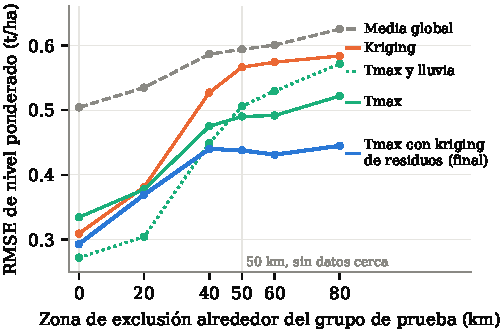
\includegraphics[width=\columnwidth]{g2_exclusion}
\caption{RMSE de nivel ponderado contra el radio de la zona de exclusión. A mayor radio, más lejos queda el municipio
de prueba del SIAP de entrenamiento más cercano.}
\label{fig:exclusion}
\end{figure}

\begin{itemize}
\item \textbf{Sin datos cerca, el ambiente supera al kriging.} Con $B = 50$\,km el kriging de vecinos tiene un RMSE
ponderado de 0.566\,t/ha. El modelo de Tmax de julio y agosto baja a 0.490 y gana en 10 de 10 repeticiones con
$p = 0.01$. El de Tmax y lluvia baja a 0.506, también con 10 de 10 y $p = 0.01$. Con el kriging de los residuos de
Tmax el error queda en 0.438 y gana en 10 de 10, ponderado y sin ponderar. Con 80\,km queda en 0.445, contra 0.584 del
kriging.
\item \textbf{Con vecinos cerca, la ventaja depende de la ponderación.} Con $B = 0$ y ponderando, el modelo de Tmax y
lluvia tiene 0.272 contra 0.309 del kriging, con 10 de 10 y $p = 0.01$. El kriging de residuos de Tmax tiene 0.293,
con 7 de 10 y $p = 0.02$. Sin ponderar, el kriging gana a todos los modelos ambientales en las 10 repeticiones, con
0.343 contra 0.411 del kriging de residuos de Tmax. Los municipios chicos tienen medias ruidosas que se parecen a las
de sus vecinos, y el clima no las explica. En los municipios con al menos 1\,000\,ha sembradas el kriging de
residuos de Tmax tiene 0.274 contra 0.307 del kriging.
\item \textbf{Por distrito, el kriging pierde su ventaja.} Al dejar fuera un DDR completo, el kriging sube a
0.503\,t/ha, cerca de la media global (0.534). El modelo de Tmax y lluvia queda en 0.305 y el kriging de residuos de
Tmax en 0.393. Parte de la ventaja del kriging venía de que el SIAP copia la cifra dentro del distrito.
\item \textbf{Sin cifras repetidas, el orden se mantiene.} Con las 862 filas sin repetir y $B = 0$, el kriging tiene
0.402, el kriging de residuos de Tmax 0.383 y el modelo de Tmax y lluvia 0.365.
\item \textbf{Más variables no ayudan.} El ridge y el lasso de 14 variables quedan cerca del kriging con $B = 0$
(0.302 ambos, contra 0.309) y le ganan solo en 4 de 10 repeticiones. Además se degradan con la distancia. Con $B = 50$\,km tienen 0.662 y 0.612, peor que la media global (0.594). La
elevación sola tampoco basta (0.631).
\end{itemize}

\textbf{Modelo final.} Por la regla fijada, el modelo de Tmax pasa contra el kriging con $B = 50$\,km. Entre las
variantes que la pasan elegimos la de menor promedio de la métrica principal en 0 y 50\,km, que es el kriging de los
residuos de Tmax, con 0.366\,t/ha. El kriging de vecinos promedia 0.438 y el modelo de Tmax solo 0.412. Lejos de los
datos se comporta como el modelo de clima y cerca corrige con el SIAP observado.

\subsection{Qué variables importan}

La Fig.~\ref{fig:importancia} muestra la importancia condicional y marginal de cada bloque.

\begin{figure}[t]
\centering
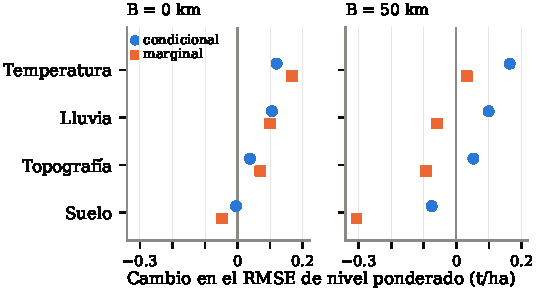
\includegraphics[width=\columnwidth]{g3_importancia}
\caption{Importancia por bloque con 99 permutaciones. Condicional, cuánto empeora el modelo de cuatro bloques al
revolver el bloque. Marginal, cuánto mejora un modelo con solo el bloque sobre la media global. Valores positivos
indican que el bloque ayuda.}
\label{fig:importancia}
\end{figure}

\begin{itemize}
\item \textbf{La temperatura es el bloque más fuerte.} Con $B = 0$, revolverla empeora el modelo en 0.120\,t/ha y sola
mejora a la media global en 0.167, ambas con $p = 0.01$. Con $B = 50$\,km es el único bloque que mejora por sí solo,
en 0.032 con $p = 0.01$.
\item \textbf{La lluvia agrega información propia.} Con $B = 0$ su importancia condicional es 0.106 y la marginal
0.100, ambas con $p = 0.01$.
\item \textbf{La topografía explica algo, pero casi todo lo comparte con la temperatura.} Sola mejora 0.070
($p = 0.01$), pero dado el resto agrega solo 0.038 ($p = 0.02$). La elevación y la Tmax de julio y agosto tienen una
correlación de $-0.80$ entre municipios.
\item \textbf{El suelo no agrega información detectable.} Con $B = 0$ su importancia condicional es $-0.005$
($p = 0.64$) y solo empeora a la media global en 0.049 ($p = 0.90$).
\item \textbf{Más bloques extrapolan mal.} Con $B = 50$\,km el modelo de cuatro bloques tiene 0.607\,t/ha, peor que la
media global (0.594).
\end{itemize}

La relación con la temperatura es fuerte y sencilla. Ajustado con todos los datos, el modelo de Tmax predice
0.79\,t/ha menos por cada grado más de Tmax media en julio y agosto. Con la lluvia en el modelo, el efecto es de
0.67\,t/ha por grado y la lluvia suma 0.15\,t/ha por cada 100\,mm entre mayo y octubre. Entre los municipios con SIAP
la Tmax de julio y agosto va de 23.0 a 25.7\,$^\circ$C y su correlación con el nivel es $-0.60$. Es una asociación
entre municipios, no un efecto causal.

\subsection{El clima del año no pronostica la cosecha}

Las anomalías del año parecen útiles en la validación espacial, pero no por el clima. La Fig.~\ref{fig:clima_anio}
compara el RMSE por municipio y año.

\begin{figure}[t]
\centering
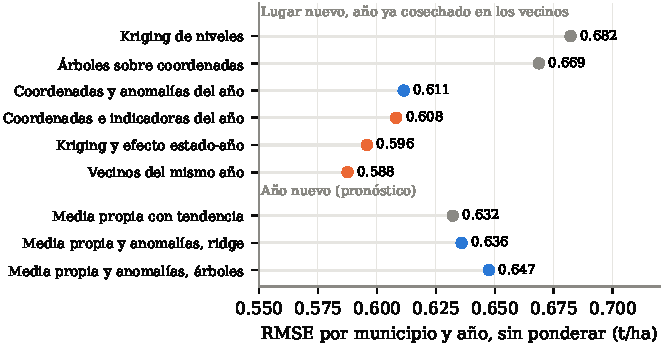
\includegraphics[width=\columnwidth]{g4_clima_anio}
\caption{RMSE por municipio y año sin ponderar. Arriba, validación espacial, donde los municipios de entrenamiento
ya traen la cosecha del mismo año. Abajo, validación por año. En azul, los modelos con anomalías de clima. En
naranja, los que usan la cosecha del año sin clima.}
\label{fig:clima_anio}
\end{figure}

\begin{itemize}
\item \textbf{En la validación espacial, las anomalías equivalen a indicadoras de año.} Un modelo de árboles de
gradiente sobre las coordenadas tiene 0.669\,t/ha. Con las anomalías baja a 0.611 y gana en 10 de 10 repeticiones.
Pero con indicadoras de año en lugar de anomalías baja a 0.608, y las anomalías solo le ganan en 3 de 10. Una
indicadora de año es una variable que vale uno en ese año y cero en los demás. Las anomalías son casi iguales en toda
la región, así que el modelo las usa para reconocer el año y copiar la cosecha de los vecinos. El kriging con el
efecto del estado en el año (0.596) y los vecinos del mismo año (0.588) hacen lo mismo sin clima.
\item \textbf{En la validación por año, las anomalías no mejoran.} La media propia de cada municipio con tendencia
tiene 0.632\,t/ha. Agregar las anomalías da 0.636 con ridge y 0.647 con árboles. Ponderando, la media propia tiene
0.603 y con anomalías y ridge 0.602, un empate. Con clima mensual no se puede pronosticar un año nuevo.
\end{itemize}

\subsection{Riesgo y cobertura}

Con la escala global, Puebla quedó con una cobertura de 0.740 con $B = 0$, debajo del mínimo de 0.75. La escala local
la sube a 0.819, así que la regla eligió la escala local.
\begin{itemize}
\item \textbf{Con datos cerca la cobertura es cercana a la nominal.} Con $B = 0$ es 0.815 sin ponderar y 0.825
ponderada. Por estado va de 0.778 en Hidalgo a 0.859 en Tlaxcala. El ancho medio del intervalo es 1.862\,t/ha.
\item \textbf{Sin datos cerca el intervalo se ensancha.} Con $B = 50$\,km la cobertura es 0.815 sin ponderar y 0.797
ponderada, con un ancho medio de 2.060\,t/ha. Hidalgo subcubre, con 0.740.
\item \textbf{La probabilidad bajo 2\,t/ha sobreestima un poco el riesgo.} Con $B = 0$ la probabilidad media es 0.475 y
la fracción observada de años bajo 2\,t/ha es 0.411. El puntaje de Brier, el error cuadrático medio de la
probabilidad, es 0.199.
\item \textbf{El rendimiento sobre sembrada se cubre igual.} Su cobertura con $B = 0$ es 0.817.
\end{itemize}

\subsection{Capa municipal}

Aplicamos el modelo final a los 486 municipios de los cuatro estados (Fig.~\ref{fig:mapas}). Solo publicamos valores
en los 268 municipios cuyo ambiente cae dentro del rango de los municipios con SIAP. Los otros 218 son sobre todo
tierras bajas y calientes donde no se siembra cebada de temporal y donde el modelo lineal extrapola. Cada municipio
con valor lleva una marca de confianza.
\begin{itemize}
\item \textbf{Alta.} El municipio tiene historia propia en el SIAP. Son 100.
\item \textbf{Media.} Sin historia propia, pero con agricultura de temporal, a no más de 25\,km de un municipio con
SIAP y dentro del dominio. El dominio pide además al menos 100\,ha de temporal y SIAP a no más de 50\,km. Son 91.
\item \textbf{Baja.} El resto de los municipios con valor. Son 77.
\end{itemize}

\begin{figure*}[t]
\centering
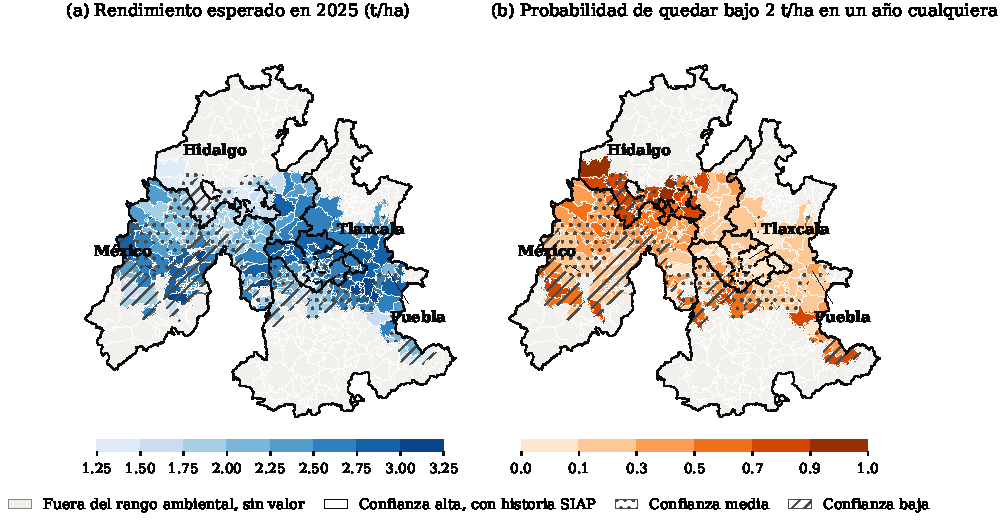
\includegraphics[width=\textwidth]{g5_mapas}
\caption{Rendimiento oficial esperado en 2025 y probabilidad de quedar bajo 2\,t/ha en un año cualquiera, por
municipio. El rayado marca la confianza media (puntos) y baja (líneas). En gris claro, los municipios fuera del rango
ambiental de los municipios con SIAP, sin valor.}
\label{fig:mapas}
\end{figure*}

\begin{itemize}
\item \textbf{El rendimiento esperado va de 1.26 a 3.16\,t/ha.} La mediana de los municipios de confianza alta es
2.53\,t/ha, con una probabilidad mediana de 0.23 de quedar bajo 2\,t/ha. El ancho mediano del intervalo es
1.90\,t/ha.
\item \textbf{Los mejores municipios con historia están en el oriente de Puebla.} San Salvador el Seco y San Juan
Atenco esperan 3.16\,t/ha, con probabilidad de 0.18 de quedar bajo 2\,t/ha.
\item \textbf{Los peores están en Hidalgo.} Huichapan espera 1.33\,t/ha, San Agustín Tlaxiaca 1.38 y Nopala de
Villagrán 1.43, con probabilidades de 0.91, 0.99 y 0.88.
\item \textbf{La marca de confianza separa a los municipios frescos sin tradición cebadera.} De los 10 municipios con
mayor rendimiento esperado, 5 son de confianza alta, 2 de media y 3 de baja. Jilotzingo (3.08\,t/ha) y Huixquilucan
(2.97) quedan en baja porque están a 37 y 47\,km del municipio con SIAP más cercano. Tlalmanalco (3.07) queda en
media porque está a 18\,km de uno, aunque solo tiene 237\,ha de temporal.
\end{itemize}

\subsection{Relación con las etiquetas del reto}

Para los 9 municipios del reto predijimos su nivel en 2025 sin usarlos en el ajuste y lo comparamos con la media de
sus parcelas por régimen (Fig.~\ref{fig:reto}). La comparación es descriptiva.

\begin{figure}[t]
\centering
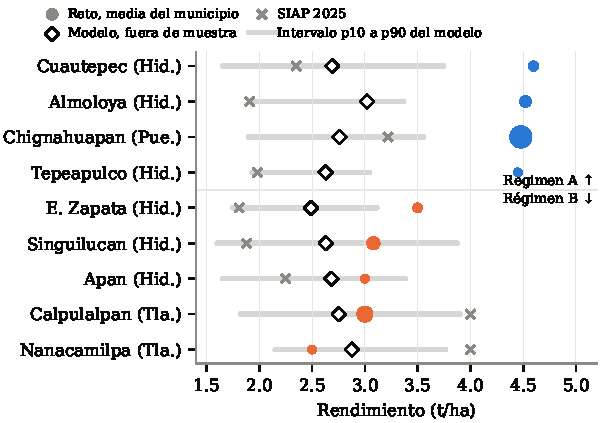
\includegraphics[width=\columnwidth]{g6_reto}
\caption{Media de las parcelas del reto por municipio (círculos, tamaño según el número de parcelas), nivel del
modelo fuera de muestra con su intervalo p10 a p90 y rendimiento del SIAP en 2025.}
\label{fig:reto}
\end{figure}

\begin{itemize}
\item \textbf{El régimen A queda muy arriba del modelo.} Sus 87 parcelas en 4 municipios promedian 4.49\,t/ha y el
modelo da 2.78, una diferencia de 1.71\,t/ha. Por municipio va de 1.50 a 1.91. El SIAP de 2025 de esos municipios
promedia 3.01.
\item \textbf{El régimen B se parece al modelo.} Sus 51 parcelas en 5 municipios promedian 3.05\,t/ha y el modelo da
2.70, una diferencia de 0.35. Por municipio va de $-0.38$ a 1.01. El SIAP de 2025 promedia 3.17.
\end{itemize}
Esto es consistente con que las etiquetas del régimen A miden otra cosa que el promedio municipal, pero no lo prueba.
